\documentclass{standalone}
\usepackage{tikz}
\usetikzlibrary{patterns, positioning}

\begin{document}
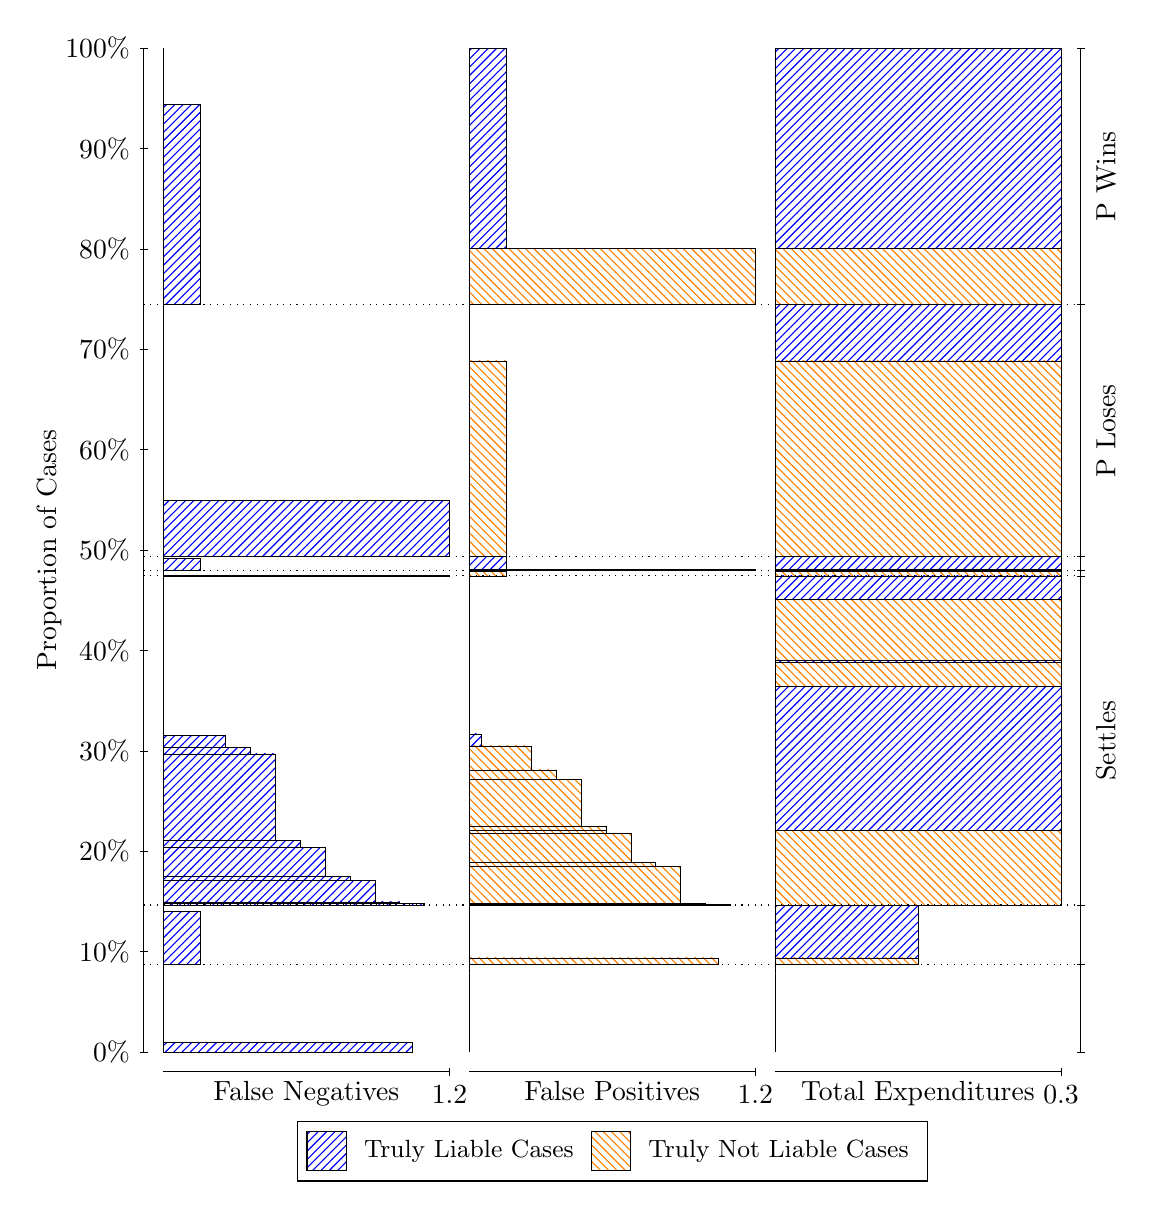
\begin{tikzpicture}
\draw[black, very thin] (1.5,1.75) -- (1.5,14.5);
\node[rotate=90, anchor=center] at (0.3, 8.125) {Proportion of Cases};
\draw[black, very thin] (1.45,1.75) -- (1.55,1.75);
\node[anchor=east] at (1.45, 1.75) {0\%};
\draw[black, very thin] (1.45,3.025) -- (1.55,3.025);
\node[anchor=east] at (1.45, 3.025) {10\%};
\draw[black, very thin] (1.45,4.3) -- (1.55,4.3);
\node[anchor=east] at (1.45, 4.3) {20\%};
\draw[black, very thin] (1.45,5.575) -- (1.55,5.575);
\node[anchor=east] at (1.45, 5.575) {30\%};
\draw[black, very thin] (1.45,6.85) -- (1.55,6.85);
\node[anchor=east] at (1.45, 6.85) {40\%};
\draw[black, very thin] (1.45,8.125) -- (1.55,8.125);
\node[anchor=east] at (1.45, 8.125) {50\%};
\draw[black, very thin] (1.45,9.4) -- (1.55,9.4);
\node[anchor=east] at (1.45, 9.4) {60\%};
\draw[black, very thin] (1.45,10.675) -- (1.55,10.675);
\node[anchor=east] at (1.45, 10.675) {70\%};
\draw[black, very thin] (1.45,11.95) -- (1.55,11.95);
\node[anchor=east] at (1.45, 11.95) {80\%};
\draw[black, very thin] (1.45,13.225) -- (1.55,13.225);
\node[anchor=east] at (1.45, 13.225) {90\%};
\draw[black, very thin] (1.45,14.5) -- (1.55,14.5);
\node[anchor=east] at (1.45, 14.5) {100\%};

\draw[black, very thin] (13.4,1.75) -- (13.4,14.5);
\draw[black, very thin] (13.35,1.75) -- (13.45,1.75);
\node[anchor=west] at (13.35, 1.75) {};
\draw[black, very thin] (13.35,2.866) -- (13.45,2.866);
\node[anchor=west] at (13.35, 2.866) {};
\draw[black, very thin] (13.35,3.616) -- (13.45,3.616);
\node[anchor=west] at (13.35, 3.616) {};
\draw[black, very thin] (13.35,7.7973) -- (13.45,7.7973);
\node[anchor=west] at (13.35, 7.7973) {};
\draw[black, very thin] (13.35,7.8618) -- (13.45,7.8618);
\node[anchor=west] at (13.35, 7.8618) {};
\draw[black, very thin] (13.35,8.039) -- (13.45,8.039);
\node[anchor=west] at (13.35, 8.039) {};
\draw[black, very thin] (13.35,11.24) -- (13.45,11.24);
\node[anchor=west] at (13.35, 11.24) {};
\draw[black, very thin] (13.35,14.5) -- (13.45,14.5);
\node[anchor=west] at (13.35, 14.5) {};

\draw[black, very thin, pattern color=blue, pattern=north east lines] (1.75,1.75) rectangle (4.9094,1.8674);
\draw[black, very thin, pattern color=orange, pattern=north west lines] (1.75,1.8674) rectangle (1.75,2.866);
\draw[black, very thin, pattern color=blue, pattern=north east lines] (1.75,2.866) rectangle (2.2239,3.5381);
\draw[black, very thin, pattern color=orange, pattern=north west lines] (1.75,3.5381) rectangle (1.75,3.616);
\draw[black, very thin, pattern color=blue, pattern=north east lines] (1.75,3.616) rectangle (5.0674,3.6405);
\draw[black, very thin, pattern color=blue, pattern=north east lines] (1.75,3.6405) rectangle (4.7514,3.6572);
\draw[black, very thin, pattern color=blue, pattern=north east lines] (1.75,3.6572) rectangle (4.4355,3.9316);
\draw[black, very thin, pattern color=blue, pattern=north east lines] (1.75,3.9316) rectangle (4.1196,3.9782);
\draw[black, very thin, pattern color=blue, pattern=north east lines] (1.75,3.9782) rectangle (3.8036,4.3523);
\draw[black, very thin, pattern color=blue, pattern=north east lines] (1.75,4.3523) rectangle (3.4877,4.4326);
\draw[black, very thin, pattern color=blue, pattern=north east lines] (1.75,4.4326) rectangle (3.1717,5.535);
\draw[black, very thin, pattern color=blue, pattern=north east lines] (1.75,5.535) rectangle (2.8558,5.623);
\draw[black, very thin, pattern color=blue, pattern=north east lines] (1.75,5.623) rectangle (2.5399,5.775);
\draw[black, very thin, pattern color=orange, pattern=north west lines] (1.75,5.775) rectangle (1.75,7.7973);
\draw[black, very thin, pattern color=blue, pattern=north east lines] (1.75,7.7973) rectangle (5.3833,7.8031);
\draw[black, very thin, pattern color=orange, pattern=north west lines] (1.75,7.8031) rectangle (1.75,7.8618);
\draw[black, very thin, pattern color=blue, pattern=north east lines] (1.75,7.8618) rectangle (2.2239,8.0227);
\draw[black, very thin, pattern color=orange, pattern=north west lines] (1.75,8.0227) rectangle (1.75,8.039);
\draw[black, very thin, pattern color=blue, pattern=north east lines] (1.75,8.039) rectangle (5.3833,8.7518);
\draw[black, very thin, pattern color=orange, pattern=north west lines] (1.75,8.7518) rectangle (1.75,11.24);
\draw[black, very thin, pattern color=blue, pattern=north east lines] (1.75,11.24) rectangle (2.2239,13.786);
\draw[black, very thin, pattern color=orange, pattern=north west lines] (1.75,13.786) rectangle (1.75,14.5);
\draw[black, very thin, pattern color=orange, pattern=north west lines] (5.6333,1.75) rectangle (5.6333,2.7486);
\draw[black, very thin, pattern color=blue, pattern=north east lines] (5.6333,2.7486) rectangle (5.6333,2.866);
\draw[black, very thin, pattern color=orange, pattern=north west lines] (5.6333,2.866) rectangle (8.7928,2.9439);
\draw[black, very thin, pattern color=blue, pattern=north east lines] (5.6333,2.9439) rectangle (5.6333,3.616);
\draw[black, very thin, pattern color=orange, pattern=north west lines] (5.6333,3.616) rectangle (8.9507,3.6275);
\draw[black, very thin, pattern color=orange, pattern=north west lines] (5.6333,3.6275) rectangle (8.6348,3.6401);
\draw[black, very thin, pattern color=orange, pattern=north west lines] (5.6333,3.6401) rectangle (8.3188,4.1108);
\draw[black, very thin, pattern color=orange, pattern=north west lines] (5.6333,4.1108) rectangle (8.0029,4.1599);
\draw[black, very thin, pattern color=orange, pattern=north west lines] (5.6333,4.1599) rectangle (7.687,4.5232);
\draw[black, very thin, pattern color=orange, pattern=north west lines] (5.6333,4.5232) rectangle (7.371,4.5653);
\draw[black, very thin, pattern color=orange, pattern=north west lines] (5.6333,4.5653) rectangle (7.371,4.6107);
\draw[black, very thin, pattern color=orange, pattern=north west lines] (5.6333,4.6107) rectangle (7.0551,5.2159);
\draw[black, very thin, pattern color=orange, pattern=north west lines] (5.6333,5.2159) rectangle (6.7391,5.3317);
\draw[black, very thin, pattern color=orange, pattern=north west lines] (5.6333,5.3317) rectangle (6.4232,5.6382);
\draw[black, very thin, pattern color=blue, pattern=north east lines] (5.6333,5.6382) rectangle (5.7913,5.7903);
\draw[black, very thin, pattern color=blue, pattern=north east lines] (5.6333,5.7903) rectangle (5.6333,7.7973);
\draw[black, very thin, pattern color=orange, pattern=north west lines] (5.6333,7.7973) rectangle (6.1072,7.856);
\draw[black, very thin, pattern color=blue, pattern=north east lines] (5.6333,7.856) rectangle (5.6333,7.8618);
\draw[black, very thin, pattern color=orange, pattern=north west lines] (5.6333,7.8618) rectangle (9.2667,7.8781);
\draw[black, very thin, pattern color=blue, pattern=north east lines] (5.6333,7.8781) rectangle (6.1072,8.039);
\draw[black, very thin, pattern color=orange, pattern=north west lines] (5.6333,8.039) rectangle (6.1072,10.527);
\draw[black, very thin, pattern color=blue, pattern=north east lines] (5.6333,10.527) rectangle (5.6333,11.24);
\draw[black, very thin, pattern color=orange, pattern=north west lines] (5.6333,11.24) rectangle (9.2667,11.953);
\draw[black, very thin, pattern color=blue, pattern=north east lines] (5.6333,11.953) rectangle (6.1072,14.5);
\draw[black, very thin, pattern color=orange, pattern=north west lines] (9.5167,1.75) rectangle (9.5167,2.7486);
\draw[black, very thin, pattern color=blue, pattern=north east lines] (9.5167,2.7486) rectangle (9.5167,2.866);
\draw[black, very thin, pattern color=orange, pattern=north west lines] (9.5167,2.866) rectangle (11.333,2.9439);
\draw[black, very thin, pattern color=blue, pattern=north east lines] (9.5167,2.9439) rectangle (11.333,3.616);
\draw[black, very thin, pattern color=orange, pattern=north west lines] (9.5167,3.616) rectangle (13.15,4.5653);
\draw[black, very thin, pattern color=blue, pattern=north east lines] (9.5167,4.5653) rectangle (13.15,6.3963);
\draw[black, very thin, pattern color=orange, pattern=north west lines] (9.5167,6.3963) rectangle (13.15,6.7029);
\draw[black, very thin, pattern color=blue, pattern=north east lines] (9.5167,6.7029) rectangle (13.15,6.7273);
\draw[black, very thin, pattern color=orange, pattern=north west lines] (9.5167,6.7273) rectangle (13.15,7.4937);
\draw[black, very thin, pattern color=blue, pattern=north east lines] (9.5167,7.4937) rectangle (13.15,7.7973);
\draw[black, very thin, pattern color=orange, pattern=north west lines] (9.5167,7.7973) rectangle (13.15,7.856);
\draw[black, very thin, pattern color=blue, pattern=north east lines] (9.5167,7.856) rectangle (13.15,7.8618);
\draw[black, very thin, pattern color=orange, pattern=north west lines] (9.5167,7.8618) rectangle (13.15,7.8781);
\draw[black, very thin, pattern color=blue, pattern=north east lines] (9.5167,7.8781) rectangle (13.15,8.039);
\draw[black, very thin, pattern color=orange, pattern=north west lines] (9.5167,8.039) rectangle (13.15,10.527);
\draw[black, very thin, pattern color=blue, pattern=north east lines] (9.5167,10.527) rectangle (13.15,11.24);
\draw[black, very thin, pattern color=orange, pattern=north west lines] (9.5167,11.24) rectangle (13.15,11.953);
\draw[black, very thin, pattern color=blue, pattern=north east lines] (9.5167,11.953) rectangle (13.15,14.5);
\draw[black, dotted] (1.5,2.866) -- (13.4,2.866);
\draw[black, dotted] (1.5,3.616) -- (13.4,3.616);
\draw[black, dotted] (1.5,7.7973) -- (13.4,7.7973);
\draw[black, dotted] (1.5,7.8618) -- (13.4,7.8618);
\draw[black, dotted] (1.5,8.039) -- (13.4,8.039);
\draw[black, dotted] (1.5,11.24) -- (13.4,11.24);
\draw[black, very thin] (1.75,1.5) -- (5.3833,1.5);
\node[anchor=north] at (3.5667, 1.5) {False Negatives};
\draw[black, very thin] (5.3833,1.45) -- (5.3833,1.55);
\node[anchor=north] at (5.3833, 1.45) {1.2};

\draw[black, very thin] (5.6333,1.5) -- (9.2667,1.5);
\node[anchor=north] at (7.45, 1.5) {False Positives};
\draw[black, very thin] (9.2667,1.45) -- (9.2667,1.55);
\node[anchor=north] at (9.2667, 1.45) {1.2};

\draw[black, very thin] (9.5167,1.5) -- (13.15,1.5);
\node[anchor=north] at (11.333, 1.5) {Total Expenditures};
\draw[black, very thin] (13.15,1.45) -- (13.15,1.55);
\node[anchor=north] at (13.15, 1.45) {0.3};



\node[black, centered, rotate=90] at (13.72, 5.7066) {Settles};


\node[black, centered, rotate=90] at (13.72, 9.6393) {P Loses};
\node[black, centered, rotate=90] at (13.72, 12.87) {P Wins};

\draw (7.449999999999999,1.5) node[draw=none] (baseCoordinate) {};
\begin{scope}[align=center]
        \matrix[scale=0.5, draw=black, below=0.5cm of baseCoordinate, nodes={draw}, column sep=0.1cm]{
            \node[rectangle, draw, minimum width=0.5cm, minimum height=0.5cm, pattern=north east lines, pattern color=blue] {}; &
            \node[draw=none, font=\small] (B) {Truly Liable Cases}; &
            \node[rectangle, draw, minimum width=0.5cm, minimum height=0.5cm, pattern=north west lines, pattern color=orange] {}; &
            \node[draw=none, font=\small] (B) {Truly Not Liable Cases}; \\
            };
\end{scope}

\end{tikzpicture}
\end{document}